\documentclass[11pt]{article}
\usepackage{amsmath,amssymb,amsfonts}
\usepackage{geometry}
\usepackage{booktabs}
\usepackage{hyperref}
\usepackage{xcolor}
\usepackage{algorithm}
\usepackage{graphicx}
\usepackage{algorithmic}
\geometry{margin=1in}
\title{So FAR, So Good: Making Your Risk Estimates Float Without Drowning}

\author{}
\date{\today}

\begin{document}
\maketitle

\tableofcontents
\newpage

\section{Introduction to Floating Absolute Risk}

\subsection{Motivation and Problem Statement}

In epidemiological studies, when analyzing categorical risk factors with more than two levels, researchers face several challenges:

\begin{enumerate}
    \item \textbf{Arbitrary reference category}: Choosing one level as baseline is often arbitrary
    \item \textbf{Inflated confidence intervals}: If the reference category has small sample size, all non-baseline CIs become inflated
    \item \textbf{Hidden comparisons}: Readers cannot calculate correct CIs for comparisons between non-baseline categories
    \item \textbf{Shared uncertainty}: All estimates share uncertainty from the reference category
\end{enumerate}

\subsection{The FAR Solution}

Easton et al. (1991) proposed treating relative risk parameters as \textit{absolute risks on a floating scale with no fixed origin}. This approach:
\begin{itemize}
    \item Assigns each level its own ``floated'' variance
    \item Treats all levels symmetrically
    \item Allows calculation of any contrast with appropriate precision
    \item Provides a ``virtually sufficient'' summary of the data
\end{itemize}

\section{Mathematical Framework}

\subsection{Notation}

Consider a risk factor with levels $0, 1, \ldots, m$ where level 0 is the reference:
\begin{align}
    \boldsymbol{\beta} &= (\beta_1, \ldots, \beta_m)^T \quad \text{(log relative risk parameters)} \\
    \hat{\boldsymbol{\beta}} &\sim N(\boldsymbol{\beta}, \hat{\boldsymbol{\Omega}}) \quad \text{(estimated parameters)}
\end{align}

where $\hat{\boldsymbol{\Omega}}$ is the estimated variance-covariance matrix from the regression model.

\subsection{The FAR Model Structure}

FAR replaces the data matrix $\hat{\boldsymbol{\Omega}}$ with a model matrix:
\begin{equation}
    \boldsymbol{\Omega} = \boldsymbol{\Lambda} + \lambda_0 \mathbf{1}\mathbf{1}^T
\end{equation}

where:
\begin{itemize}
    \item $\boldsymbol{\Lambda} = \text{diag}(\lambda_1, \ldots, \lambda_m)$ contains the floated variances
    \item $\lambda_0$ is the floated variance for the reference level
    \item $\mathbf{1}$ is a vector of ones
\end{itemize}

\subsubsection{Matrix Structure Example}
For $m = 3$:
\begin{equation}
    \boldsymbol{\Omega} = \begin{pmatrix}
        \lambda_1 + \lambda_0 & \lambda_0 & \lambda_0 \\
        \lambda_0 & \lambda_2 + \lambda_0 & \lambda_0 \\
        \lambda_0 & \lambda_0 & \lambda_3 + \lambda_0
    \end{pmatrix}
\end{equation}

\subsection{Latent Variable Interpretation}

The FAR structure can be motivated through latent absolute risks:

Let $\hat{\alpha}_i$ be the (unobserved) absolute risk estimate for level $i$, with:
\begin{align}
    \hat{\alpha}_i &\sim N(\alpha_i, \lambda_i) \quad \text{independently} \\
    \hat{\beta}_i &= \hat{\alpha}_i - \hat{\alpha}_0 \quad \text{(observed relative risks)}
\end{align}

This gives:
\begin{align}
    \text{Var}(\hat{\beta}_i) &= \text{Var}(\hat{\alpha}_i - \hat{\alpha}_0) = \lambda_i + \lambda_0 \\
    \text{Cov}(\hat{\beta}_i, \hat{\beta}_j) &= \text{Var}(\hat{\alpha}_0) = \lambda_0
\end{align}

\subsection{Floating Confidence Intervals}

The floating CI for level $i$ is:
\begin{equation}
    \hat{\beta}_i \pm 1.96\sqrt{\lambda_i}
\end{equation}

This is a CI for $\gamma_i = \alpha_i - \hat{\alpha}_0$, where:
\begin{itemize}
    \item $\alpha_i$ is the true absolute risk at level $i$
    \item $\hat{\alpha}_0$ is the estimated absolute risk at reference (a random variable!)
\end{itemize}

\section{Estimation Methods}

\subsection{The Heuristic Method (Easton et al., 1991)}

\begin{equation}
    \hat{\lambda}_0^{\text{heuristic}} = \frac{1}{m(m-1)} \sum_{i=1}^m \sum_{j \neq i} \hat{\Omega}_{ij}
\end{equation}

This uses equal weights for all off-diagonal elements.

\subsection{The Improved Method (Plummer, 2004)}

Minimizes the Kullback-Leibler divergence:
\begin{equation}
    D = \text{tr}(\hat{\boldsymbol{\Omega}}\boldsymbol{\Omega}^{-1}) - \log|\hat{\boldsymbol{\Omega}}\boldsymbol{\Omega}^{-1}| - m
\end{equation}

This gives:
\begin{equation}
    \lambda_0 = \frac{\sum_{i=1}^m \sum_{j=1}^m w_i(\hat{\Omega}_{ij} - \Lambda_{ij})w_j}{(\sum_{i=1}^m w_i)^2}
\end{equation}

where $w_i = 1/\lambda_i$ (weights inversely proportional to variance).

\subsection{Iterative Algorithm}

\begin{algorithm}
\caption{FAR Estimation Algorithm}
\begin{algorithmic}
\STATE \textbf{Initialize:} $\hat{\Omega}_{00}^{(0)}, \hat{\Omega}_{0i}^{(0)}$ using heuristic estimates
\REPEAT
    \STATE \textbf{Step 1:} Given $\boldsymbol{\Lambda}^*$, update augmented data matrix:
    \STATE $\quad \hat{\Omega}_{00} = \frac{1}{S} + \frac{\sum_j \sum_k w_j \hat{\Omega}_{jk} w_k}{S^2}$
    \STATE $\quad \hat{\Omega}_{0i} = \sum_j w_j \hat{\Omega}_{ji}$ for $i = 1, \ldots, m$
    \STATE \textbf{Step 2:} Given augmented data matrix, update variances:
    \STATE $\quad \lambda_0 = \hat{\Omega}_{00}$
    \STATE $\quad \lambda_i = \hat{\Omega}_{00} - 2\hat{\Omega}_{0i} + \hat{\Omega}_{ii}$ for $i = 1, \ldots, m$
\UNTIL{convergence}
\end{algorithmic}
\end{algorithm}

\section{Model Adequacy Assessment}

\subsection{Relative Standard Errors}

For any contrast $\mathbf{c}^T\boldsymbol{\beta}^*$:
\begin{equation}
    \text{Relative SE} = \frac{\sqrt{\mathbf{c}^T\boldsymbol{\Omega}\mathbf{c}}}{\sqrt{\mathbf{c}^T\hat{\boldsymbol{\Omega}}\mathbf{c}}}
\end{equation}

\subsection{Error Limits Interpretation}

The error limits $[\ell_{\min}, \ell_{\max}]$ represent:
\begin{itemize}
    \item $\ell_{\min}$: Maximum underestimation of any contrast SE
    \item $\ell_{\max}$: Maximum overestimation of any contrast SE
\end{itemize}

\begin{table}[h]
\centering
\caption{Coverage probabilities of nominal 95 per cent confidence intervals.}
\begin{tabular}{cc}
\hline
Relative error in length (\%) & Coverage probability (\%) \\
\hline
$-20$ & 88.3 \\
$-10$ & 92.2 \\
$-5$ & 93.7 \\
0 & 95.0 \\
$+5$ & 96.0 \\
$+10$ & 96.9 \\
$+20$ & 98.1 \\
\hline
\end{tabular}
\end{table}

As shown in the table above (adapted from Plummer, 2004), the coverage probability of nominal 95\% confidence intervals depends on the accuracy of the standard error estimates. When FAR underestimates the standard error by 20\% (relative error = -20\%), the actual coverage drops to 88.3\%. Conversely, when FAR overestimates by 20\%, the coverage increases to 98.1\%. For practical applications, relative errors within $\pm 5\%$ yield excellent performance with coverage probabilities close to the nominal 95\% level.

\subsection{Calculating Error Limits}

The error limits $[\ell_{\min}, \ell_{\max}]$ are obtained by considering \textit{all possible} contrasts:

\begin{enumerate}
    \item For each possible contrast vector $\mathbf{c}$ (where $\sum c_i = 0$), calculate:
    \begin{equation}
        \text{Relative SE}(\mathbf{c}) = \frac{\sqrt{\mathbf{c}^T\boldsymbol{\Omega}\mathbf{c}}}{\sqrt{\mathbf{c}^T\hat{\boldsymbol{\Omega}}\mathbf{c}}}
    \end{equation}
    
    \item Find the minimum across all contrasts:
    \begin{equation}
        \ell_{\min} = \min_{\mathbf{c}: \sum c_i = 0} \text{Relative SE}(\mathbf{c})
    \end{equation}
    
    \item Find the maximum across all contrasts:
    \begin{equation}
        \ell_{\max} = \max_{\mathbf{c}: \sum c_i = 0} \text{Relative SE}(\mathbf{c})
    \end{equation}
\end{enumerate}

In practice, these bounds are computed efficiently using the eigenvalues of the matrix $\hat{\boldsymbol{\Omega}}^{-1}\boldsymbol{\Omega}$:
\begin{itemize}
    \item $\ell_{\min} = \lambda_m^{1/2}$ (square root of smallest eigenvalue)
    \item $\ell_{\max} = \lambda_1^{1/2}$ (square root of largest eigenvalue)
\end{itemize}

This ensures we capture the worst-case performance of FAR across \textit{all possible comparisons}, not just pairwise comparisons. For example, with error limits [0.92, 1.08], FAR may underestimate some contrast's SE by up to 8\% and overestimate others by up to 8\%.
\section{Special Cases and Extensions}

\subsection{The Three-Level Factor Case}

\textbf{Key Result:} With $K = 3$ levels, FAR provides an \textit{exact} fit:

\begin{itemize}
    \item 2×2 covariance matrix → 3 unique elements
    \item FAR model → 3 parameters ($\lambda_0, \lambda_1, \lambda_2$)
    \item 3 equations, 3 unknowns → exact solution
    \item Error limits = [1.00, 1.00]
\end{itemize}

This holds regardless of how the variance-covariance matrix was generated:
\begin{itemize}
    \item Standard errors
    \item Clustered/robust standard errors
    \item Mixed effects models
\end{itemize}

\subsection{Factors with $K > 3$ Levels}

For $K$ categories:
\begin{itemize}
    \item Unique covariance elements: $K(K-1)/2$
    \item FAR parameters: $K$
    \item Perfect fit requires: $K \geq K(K-1)/2$
\end{itemize}

Only $K \leq 3$ satisfies this constraint.

\subsection{FAR with Clustered Standard Errors}

FAR can work with clustered SEs when:
\begin{enumerate}
    \item \textbf{Within-cluster randomization} with balanced allocation
    \item \textbf{Weak clustering} (ICC $< 0.05$)
    \item All treatment pairs share clusters equally
\end{enumerate}

The clustered covariance becomes:
\begin{equation}
    \hat{\boldsymbol{\Omega}}_{\text{clustered}} = \hat{\boldsymbol{\Omega}}_{\text{independent}} + \tau^2 \mathbf{M}
\end{equation}

If $\mathbf{M} \approx \mathbf{1}\mathbf{1}^T$, then FAR structure is preserved with $\lambda_0^{\text{effective}} = \lambda_0 + \tau^2$.

\subsection{Reference Category Independence}

Changing the reference category:
\begin{itemize}
    \item Changes the parameterization
    \item Changes individual $\lambda$ values
    \item Does NOT change relative SEs for any contrast
    \item Does NOT change model adequacy
\end{itemize}

\section{Practical Examples}

\subsection{Example 1: Simple 3-Level Factor}

Data: Risk factor with levels A, B, C (reference = A)
\begin{equation}
    \hat{\boldsymbol{\Omega}} = \begin{pmatrix}
        0.04 & 0.02 \\
        0.02 & 0.05
    \end{pmatrix}
\end{equation}

FAR solution:
\begin{align}
    \lambda_0 &= 0.02 \\
    \lambda_B &= 0.04 - 0.02 = 0.02 \\
    \lambda_C &= 0.05 - 0.02 = 0.03
\end{align}

Floating CIs:
\begin{itemize}
    \item Level A: $0 \pm 1.96\sqrt{0.02} = [-0.277, 0.277]$
    \item Level B: $0.5 \pm 1.96\sqrt{0.02} = [0.223, 0.777]$
    \item Level C: $1.0 \pm 1.96\sqrt{0.03} = [0.660, 1.340]$
\end{itemize}

\subsection{Example 2: When FAR Fails (Table II from Paper)}

Two trials with different treatment allocations:
\begin{itemize}
    \item Trial I: Treatments A, B, C
    \item Trial II: Treatments A, D
\end{itemize}

True covariance structure:
\begin{equation}
    \text{Cov}(\hat{\beta}_B, \hat{\beta}_C) = 0.00624, \quad
    \text{Cov}(\hat{\beta}_B, \hat{\beta}_D) = 0, \quad
    \text{Cov}(\hat{\beta}_C, \hat{\beta}_D) = 0
\end{equation}

FAR assumes all equal to $\lambda_0$ → Poor fit!

\subsection{Example 3: Real Data Application}

From the GAM analysis:
\begin{verbatim}
water_landform (5 levels):
  lake_beach        0.0000  (0.11082)  Reference
  lake_marsh        0.3570  (0.08386)  
  pond/swamp        0.5824  (0.11281)  
  rice_paddy        0.5733  (0.32346)  
  river/river_marsh 0.5220  (0.13588)  
  
Error limits: [0.92, 1.08]
\end{verbatim}

\begin{figure}
    \centering
    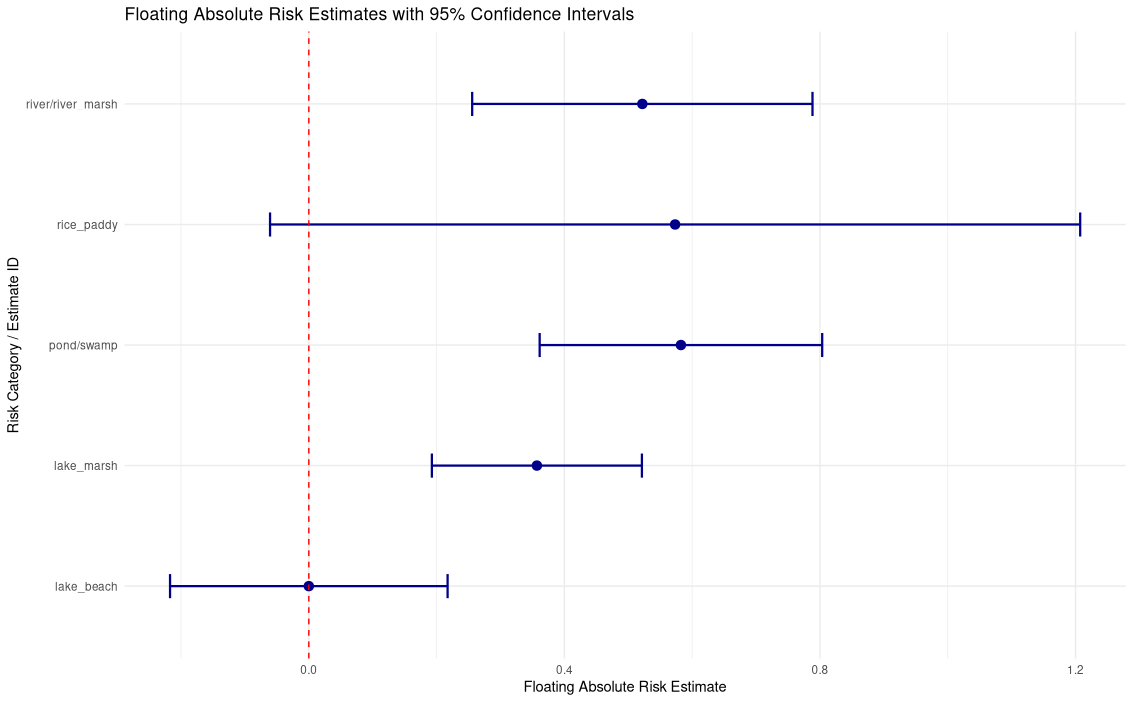
\includegraphics[width=0.9\linewidth]{overviews//FAR-clustere-SE//figs/lake_beach_ref.png}
    \caption{FAR with Lake Beach as Reference}
    \label{fig:lakembeach_ref}
\end{figure}

\begin{figure}
    
    \centering
    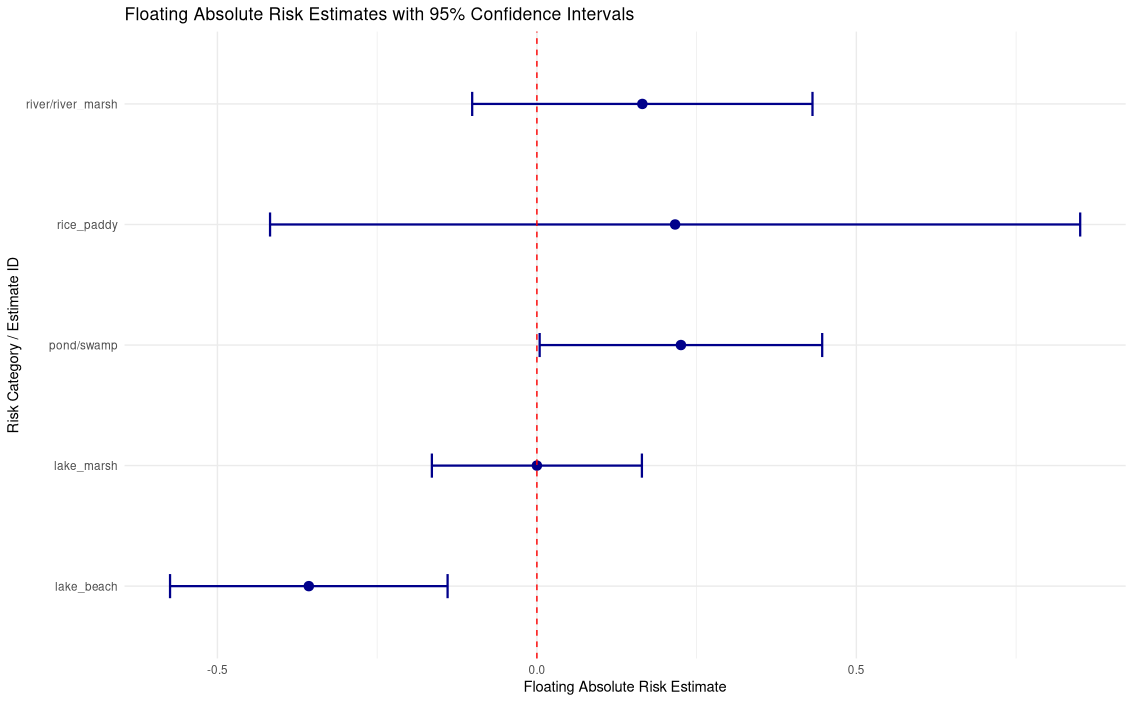
\includegraphics[width=0.9\linewidth]{overviews/FAR-clustere-SE/figs/lake_marsh_ref.png}
    \caption{FAR with Lake Marsh as Reference}
    \label{fig:lakemarsh_ref}
\end{figure}

Interpretation:
\begin{itemize}
    \item Error limits show $\pm 8\%$ accuracy → acceptable
    \item Rice paddy has high uncertainty (likely small sample)
    \item A visual plot of the FAR estimates shows that basically choosing the Reference category just shifts the vertical line \autoref{fig:lakembeach_ref} and \autoref{fig:lakemarsh_ref}
\end{itemize}

\section{FAQs about FARs}

\subsection{Q1: When does FAR not work well?}

\textbf{A:} FAR fails when the covariance structure violates the constant off-diagonal assumption:

\begin{enumerate}
    \item \textbf{Different correlation patterns}: Some pairs highly correlated, others not
    \item \textbf{Confounding by subgroups}: E.g., treatments clustered by site
    \item \textbf{Very unbalanced designs}: Extreme sample size differences
    \item \textbf{Hierarchical structures}: Natural groupings with different within/between correlations
\end{enumerate}

\subsection{Q2: What do the weights in the improved method represent?}

\textbf{A:} The weights $w_i = 1/\lambda_i$ down-weight high-variance components:

\begin{equation}
    \lambda_0 = \frac{\sum_{i,j} w_i \hat{\Omega}_{ij} w_j}{(\sum_i w_i)^2}
\end{equation}

Intuition: Imprecise estimates shouldn't dominate the estimate of shared baseline uncertainty.

\subsection{Q3: How do I interpret the reference level CI?}

\textbf{A:} The CI for the reference level represents uncertainty in $\gamma_0 = \alpha_0 - \hat{\alpha}_0$:
\begin{itemize}
    \item NOT the sampling variability in $\hat{\beta}_0$ (which is 0 by definition)
    \item It quantifies uncertainty in the baseline risk level. For example: \textit{If we had a hypothetical new study with infinite data, the log risk difference between that study's non-smokers and our study's non-smokers would fall in [-0.28, 0.28] with 95\% probability}
    \item In 95\% of studies, this interval contains 0
    \item Allows honest representation of uncertainty in all groups
\end{itemize}

\subsection{Q4: Can I use FAR with mixed effects models?}

\textbf{A:} Yes! Extract the variance-covariance matrix:
\begin{verbatim}
vcov_matrix <- vcov(mixed_model)
# Apply FAR to this matrix
\end{verbatim}

For 3-level factors, you still get perfect fit regardless of model complexity.

\subsection{Q5: How do clustered standard errors affect FAR?}

\textbf{A:} FAR works with clustered SEs when:
\begin{itemize}
    \item Treatments are randomized \textit{within} clusters
    \item All treatment pairs share clusters equally
    \item ICC is low ($< 0.05$)
\end{itemize}

Check by examining off-diagonal variation:
\begin{equation}
    \text{CV} = \frac{\text{SD(off-diagonals)}}{\text{Mean(off-diagonals)}} < 0.2 \implies \text{FAR appropriate}
\end{equation}

\subsection{Q6: What if I change the reference category?}

\textbf{A:} Changing reference affects parameters but NOT inference:
\begin{itemize}
    \item Individual $\lambda$ values change
    \item Floated variance for new reference differs
    \item Relative SEs for all contrasts remain identical
    \item Model adequacy (error limits) unchanged
\end{itemize}

\subsection{Q7: How do I calculate a specific contrast?}

\textbf{A:} For contrast between levels $i$ and $j$:
\begin{align}
    \text{Estimate} &= \hat{\beta}_i - \hat{\beta}_j \\
    \text{SE} &= \sqrt{\lambda_i + \lambda_j} \\
    \text{95\% CI} &= (\hat{\beta}_i - \hat{\beta}_j) \pm 1.96\sqrt{\lambda_i + \lambda_j}
\end{align}

\section{Summary and Recommendations}

\subsection{Key Takeaways}

\begin{enumerate}
    \item FAR provides symmetric treatment of all factor levels
    \item Perfect fit guaranteed for 3-level factors
    \item Approximation quality measurable via error limits
    \item Works with any variance estimation method (extract proper vcov)
    \item Reference choice affects parameters but not inference
\end{enumerate}

\subsection{Decision Framework}

\begin{table}[h]
\centering
\caption{Coverage probabilities of nominal 95 per cent confidence intervals.}
\begin{tabular}{cc}
\hline
Relative error in length (\%) & Coverage probability (\%) \\
\hline
$-20$ & 88.3 \\
$-10$ & 92.2 \\
$-5$ & 93.7 \\
0 & 95.0 \\
$+5$ & 96.0 \\
$+10$ & 96.9 \\
$+20$ & 98.1 \\
\hline
\end{tabular}
\end{table}

As shown in the table above (adapted from Plummer, 2004), when making the decision about adequacy of the FAR method consider the problem at hand. As a rule of thumb underestimation of the standard error (less conservative estimates, narrower confidence intervals) is probably worse in many cases than being more conservative (overestimation, positive relativ error length)

\subsection{Best Practices}

\begin{enumerate}
    \item Always report error limits
    \item For critical contrasts, verify relative SEs
    \item With clustered data, check off-diagonal homogeneity
    \item Consider reference category choice for numerical stability
    \item Document any model complexity (clustering, weights, etc.)
\end{enumerate}



\end{document}